% !TeX spellcheck = it_IT
% !TEX TS-program = pdflatex
% !TEX root = ../main.tex


% ********************************************************************
\section{Prototipo}
\label{sec:prototipo}
% ********************************************************************

\subsection{Login e autenticazione}

\subsection{Dashboard donatore}

\begin{figure}[h]
	\centering
	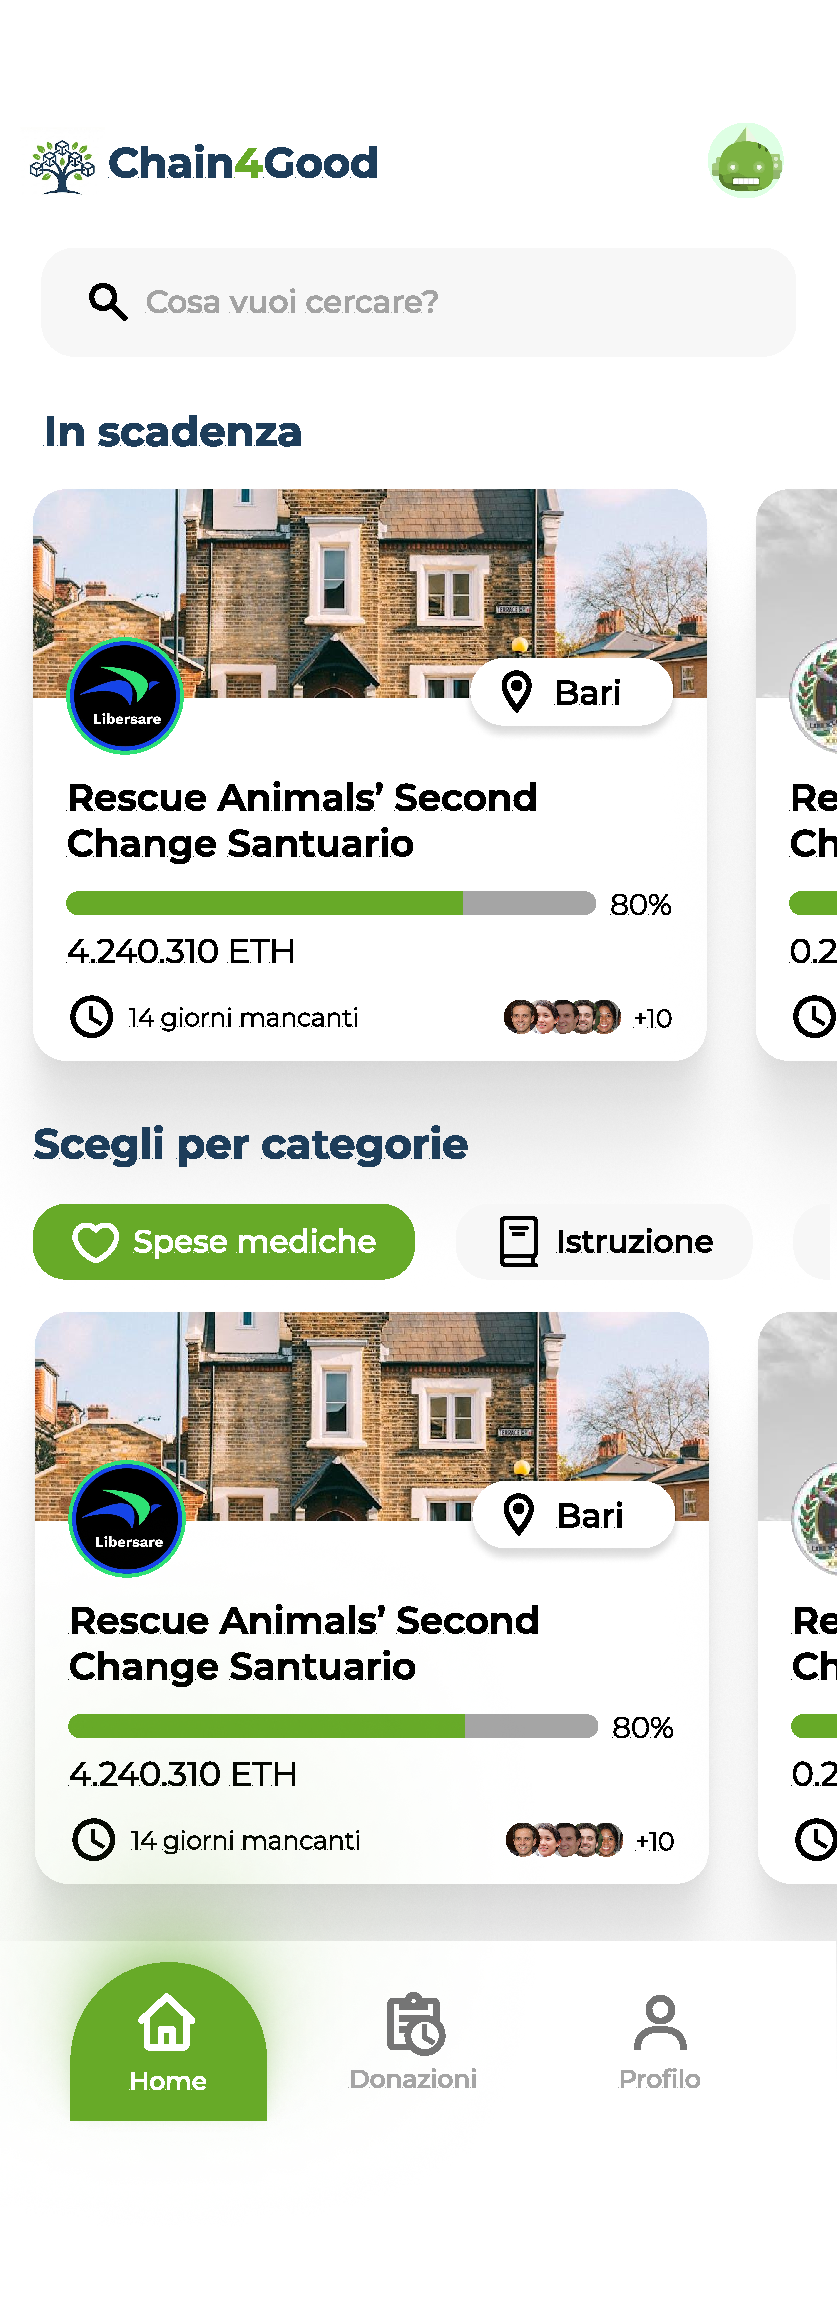
\includegraphics[width=0.45\textwidth]{images/home_utente.pdf}
	\caption{Dashboard del donatore}
	\label{fig:dashboard-donatore}
\end{figure}


\subsection{Creazione progetto}
%La creazione di un progetto consiste nell'inserimento, da parte di un Ente riconosciuto, di tutte le informazioni necessarie 




\begin{figure}[h]
	\centering
	\begin{minipage}{0.46\textwidth}
		\centering
		\includegraphics[width=\textwidth]{images/nuovo_progetto1.pdf}
	\end{minipage}
	\hspace{0.9cm}
	\begin{minipage}{0.46\textwidth}
		\centering
		\includegraphics[width=\textwidth]{images/nuovo_progetto2.pdf}
	\end{minipage}
	\caption{Inserimento di un nuovo progetto}
	\label{fig:Inserimento progetto}
\end{figure}





\subsection{Inserimento e valutazione spesa}
\begin{figure}[h]
	\centering
	\begin{minipage}{0.46\textwidth}
		\centering
		\includegraphics[width=\textwidth]{images/nuova_spesa.pdf}
	\end{minipage}
	\hspace{0.9cm}
	\begin{minipage}{0.46\textwidth}
		\centering
		\includegraphics[width=\textwidth]{images/valutazione_spesa.pdf}
	\end{minipage}
	\caption{Valutazione di una richiesta di spesa}
	\label{fig:valutazione-spesa}
\end{figure}

